\documentclass[nynorsk,14pt]{beamer}
\usepackage[utf8]{inputenc}
\usepackage[T1]{fontenc}
\usepackage{graphicx}
\usepackage{babel}

\usetheme{Warsaw}

\title[Bacheloroppgåve 20E 2013]{Dynamisk Nettverksbrannmur}
\subtitle{Bacheloroppgåve 20E}
\author[E.Gjærde, S.O.Undal] {Espen Gjærde \and Svein Ove Undal}
\institute[Høgskolen i Sør-Trøndelag]{
		HiST\\
		Avdeling for Informatikk og e-Læring	
}
\date{Mai 2013}
	
\begin{document}	

\frame{\titlepage}

\begin{frame}
	\tableofcontents
\end{frame}
\section{Oppgåvestillar}
\begin{frame} % Oppgåvestillar
	\frametitle{Oppgåvestillar}
		\begin{alertblock}{Eiga oppgåve}
			Eiga oppgåve laga av \emph{Svein Ove Undal}.
		\end{alertblock}
		\begin{itemize}
			\item Autentisering av brukarar
			\item Rettferdig fordeling av bandbreidde
		\end{itemize}
		\\ ~
	\begin{columns}[t]
		\begin{column}[T]{5cm}
		\alert {Utviklarar} \\
		Espen Gjærde \\
		Svein Ove Undal \\ ~ \\
		\end{column}		
		\begin{column}[B]{5cm}
		\alert{Rettleiar} \\	Helge Hafting
		\end{column}
	\end{columns}
\end{frame}
\section{Oppgåva}
\subsection{Problemstilling}
\begin{frame} % Problemstilling
	\frametitle{Problemstilling}
	 Lage eit system som automatisk og i sanntid kan avgrense hastigheit og antall oppkoplingar for kvar brukar. \\ ~ \\
	Kun avgrense brukarar dersom aktiviteten går ut over andre.
\end{frame}
\subsection{Grunngjeving av val}
\begin{frame} % Kvifor denne oppgåva?
	\frametitle{Kvifor denne oppgåva?}
	Oppgåva kombinerer fleire spennande fagfelt, mellom anna Linux Systemdrift, Nettverksteknologi og Nettverksikkerhet. 
	\\ ~ \\
	Oppgåve som var open for utvikling og idéar
	\\ ~ \\
	
\end{frame}
\subsection{Løysinga}
\begin{frame} % Løysing
	\frametitle{Korleis vart oppgåva løyst?}
	\begin{columns}[t]
	\begin{column}[T]{8cm}
		\begin{itemize}
			\item Vidareføring av haustprosjekt.
			\item Captive-Portal for autentisering.
			\item Python som kodespråk
			\item Django for dynamiske nettsider
			\item Linux - spesielt nettverksverktøya
			\item Apache webserver 
		\end{itemize}
	\end{column}
	\begin{column}[T]{4cm}
	\begin{flushright}
		
\includegraphics[scale=0.06]{imgs/python.png} \\
		
\includegraphics[scale=0.2]{imgs/django_logo.png} \\
		
\includegraphics[scale=0.05]{imgs/tux-trans.png}
		
\includegraphics[scale=0.1]{imgs/debian-logo.jpg}
	\end{flushright}
	\end{column}
	\end{columns}

\end{frame}

\section{Resultatet}
\subsection*{Produktet}
\begin{frame} % Resultat 1: oppsum.
	\frametitle{Resultat}
	Vi har oppnådd 
	\begin{itemize}
		\item Automagisk lastbalansering
		\item Autentisering via nettside
		\item Grafisk brukargrensesnitt
		\item CLI og WebUI for administrasjon
	\end{itemize}

\end{frame}
\subsection*{Brukarsida}
\begin{frame} %  Klient - login
	\frametitle{Tvungen pålogging}
	\small{Klientane vil automatisk verte sendt til påloggingsida om dei ikkje er authentisert.}
	\begin{figure}
	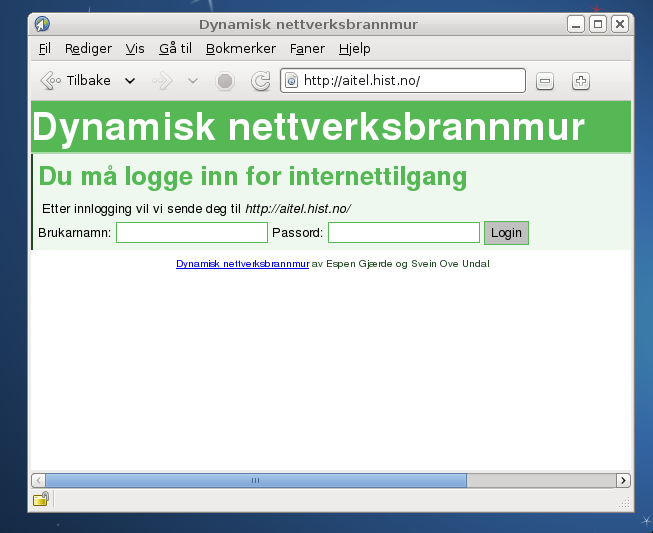
\includegraphics[scale=0.24]{imgs/innlogging.png} 
	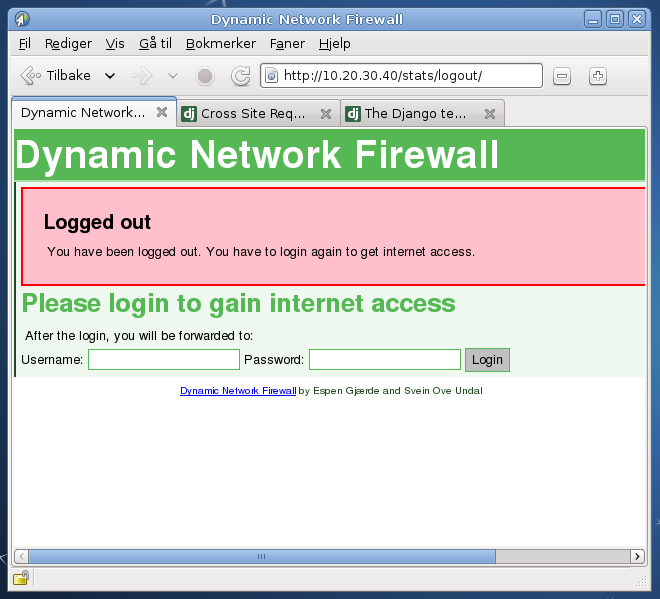
\includegraphics[scale=0.21]{imgs/user_logedout.png}
	\end{figure}
\end{frame}
\begin{frame}
	\frametitle{Statistikk}
	\small{Etter dette vil nettoppslag mot DNF-systemet sende brukaren til ei statistikk-side.}
	\begin{figure}
		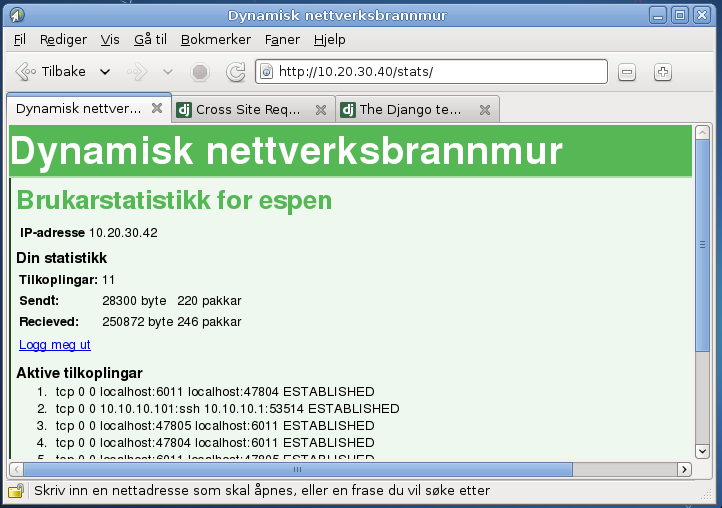
\includegraphics[scale=0.22]{imgs/user_stats.png} 
		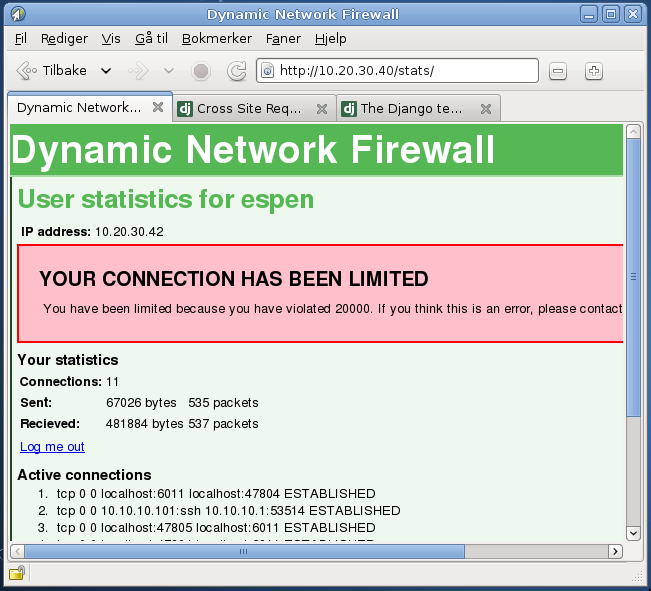
\includegraphics[scale=0.2]{imgs/user_stats_restricted.png}	
	\end{figure}
\end{frame}
\subsection*{Administrajonsida}
\begin{frame} % Resultat
	\frametitle{CLI - kommandogrensesnitt}
	\small{Frå terminalen på ei maskin som kjører systemet, kan ein bruke kommandoen \alert{dynfw}}
	\begin{figure}
	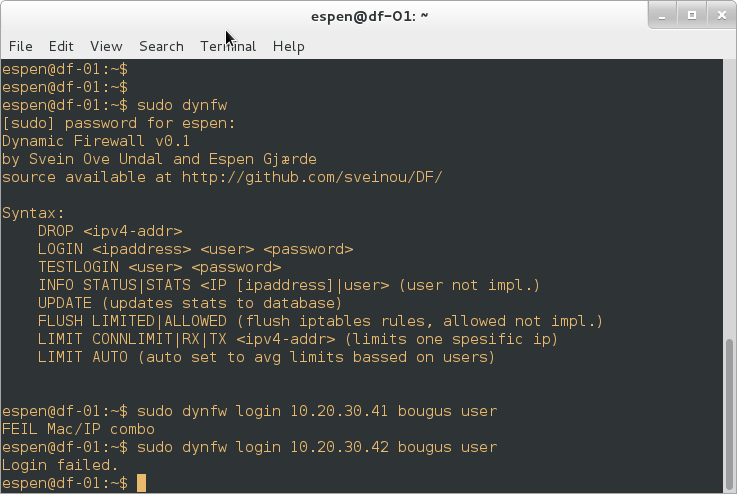
\includegraphics[scale=0.3]{imgs/dynfw_cli.png}
	\end{figure}
\end{frame}
\begin{frame} % Resultat
	\frametitle{Administrasjonspanelet}
	\small{Hovudsida for administrasjonspanelet gir ei oversikt over innstillingane sett i innstililngsfila}
	\begin{figure}
		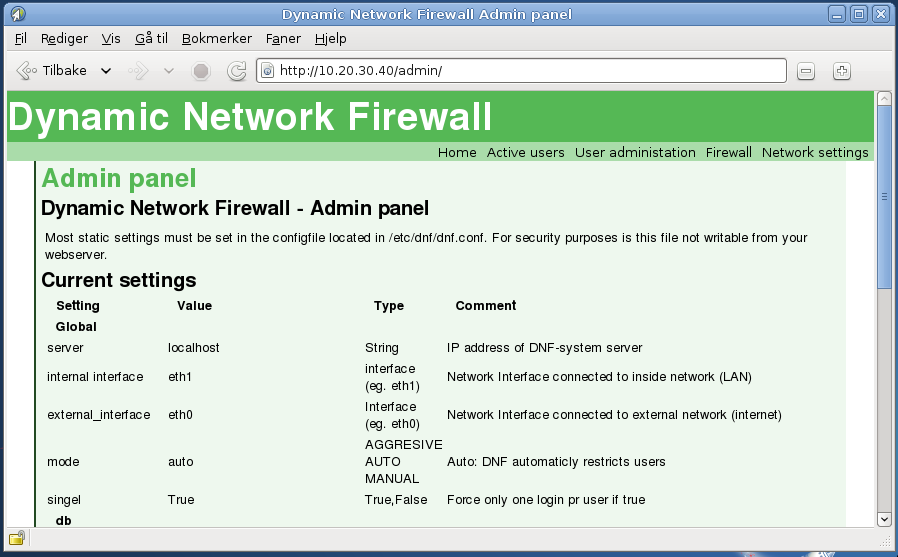
\includegraphics[scale=0.3]{imgs/admin_home.png}
	\end{figure}
\end{frame}
\begin{frame} % Resultat
	\frametitle{Administrasjonspanel}
	\begin{figure}
		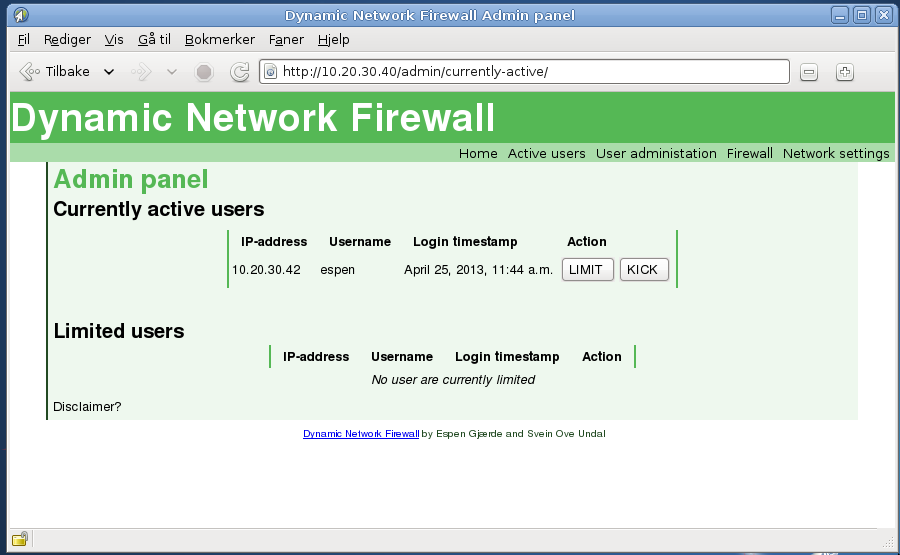
\includegraphics[scale=0.18]{imgs/admin_users.png}
		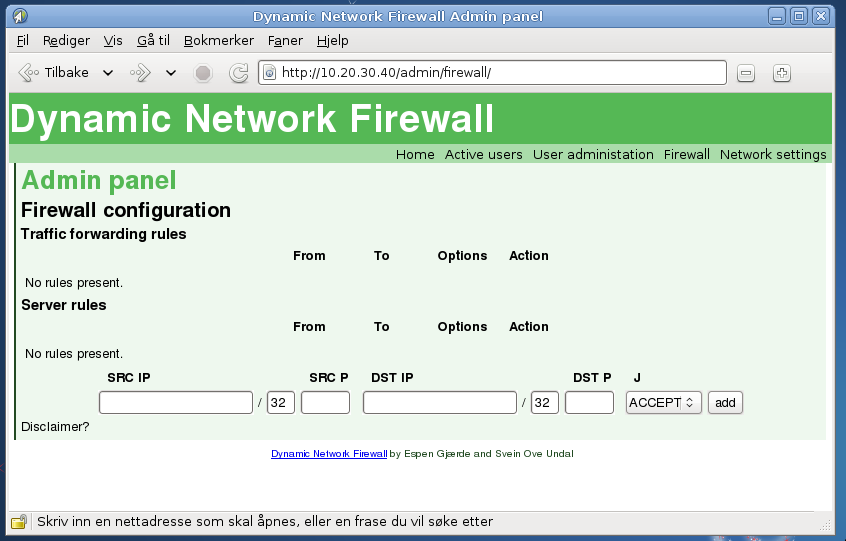
\includegraphics[scale=0.19]{imgs/custom_firewall.png} \\
		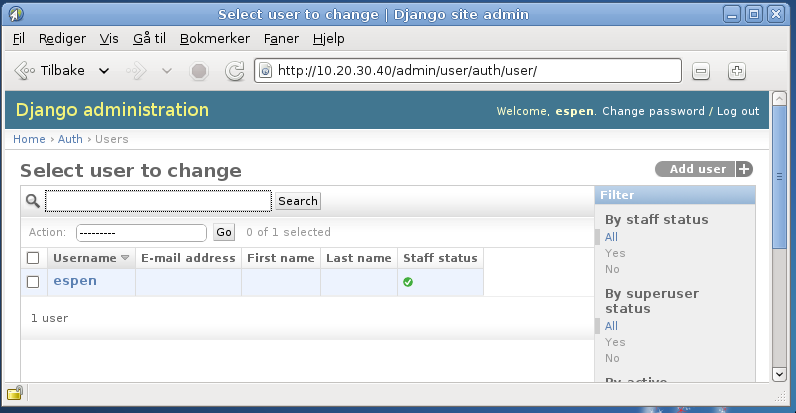
\includegraphics[scale=0.18]{imgs/django_user.png}
	\end{figure}
\end{frame}
\section{Vidare arbeid}
\begin{frame} % Vidare arbeid
	\frametitle{Vidare arbeid}
	Naturleg vidareutvikling
	\begin{itemize}
		\item Kompabilitet med IEEE 802.1x
		\item Utvikle systemet i retning av eit NMS
	\end{itemize}
\end{frame}

\end{document}
